
\section{右伴随右逆伴随}\label{sec:rajri-quasi-categories}

据我们所知，拟范畴之间的\trRightAdjoint\trRightInverse\trAdjunction{}尚未受到
多少关注。尽管如此，我们不妨驻足于此，确立这类\trAdjunction{}的一个有用的%
解析刻画，它将帮助我们比较其余各种综合定义与解析定义。

\begin{lemma}\label{lem:rajri-lifting}
拟范畴之间的\trIsofibration{} $f\colon B\twoheadrightarrow A$ 容许一个%
\trRightAdjoint\trRightInverse，当且仅当对每个\trElement{} $a\colon 1\to A$，
都存在一个满足 $fua=a$ 的\trElement{} $ua\colon 1\to B$，它具有如下性质：
任何形如下式且带 $n\ge 1$ 的\trLifting{}问题都有解
\begin{rveq}\label{eq:rajri-lifting}
\begin{tikzpicture}[x=1.9em,y=1.4em]
  \node (o)  at (0,1.4)    {$1$};
  \node (pd) at (3.4,1.4)  {$\partial\Delta[n]$};
  \node (b)  at (7.4,1.4)  {$B$};
  \node (dn) at (3.4,-1.2) {$\Delta[n]$};
  \node (a)  at (7.4,-1.2) {$A$};
  \draw[->] (o) -- node[below]{$\scriptstyle\{n\}$} (pd);
  \draw[->] (pd) -- (b);
  \draw[->] (o) to[bend left=28] node[above,pos=0.5]{$\scriptstyle ua$} (b);
  \draw[right hook->] (3.4,1.05) -- (3.4,-0.85);
  \draw[->] (b) -- node[right]{$\scriptstyle f$} (a);
  \draw[->] (dn) -- (a);
  \draw[->,dashed] (3.75,-0.95) -- (7.0,1.1);
\end{tikzpicture}
\end{rveq}
\end{lemma}

\providecommand{\rvTranspose}[1]{\ulcorner #1\urcorner}%

\begin{proof}
若 $f\colon B\twoheadrightarrow A$ 是拟范畴之间的一个\trIsofibration，容许一个%
\trRightAdjoint\trRightInverse，则由\cref{lem:rajri-fibered-adjunction}，其%
\trRightAdjoint{} $u$ 可以选取使得\trCounit{} $\epsilon\colon fu=\mathrm{id}_{A}$%
为恒等，且该\trAdjunction{}纤维化于 $A$ 之上。在此情形，%
\cref{prop:adjunction-as-fibered-equivalence}的诱导\trFiberedEquivalence{}%
$\rvTranspose{\epsilon\circ f(-)}\colon\mathrm{Hom}_{B}(B,u)\rightsquigarrow\mathrm{Hom}_{A}(f,A)$ 由\cref{prop:maps-between-commas}所定义的、$f$ 在诸%
\trCommaInfinityCategory{}之间诱导的那个映射所表示。
\begin{center}
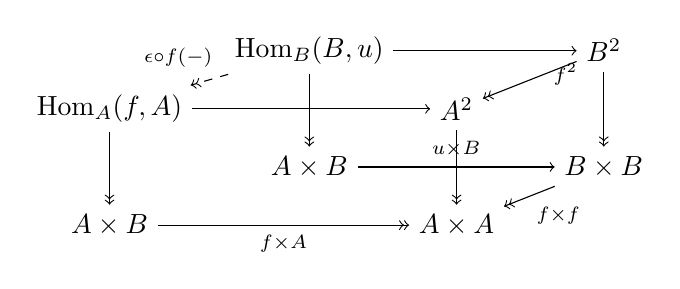
\begin{tikzpicture}[x=1.9em,y=1.5em]
  \node (hbu) at (2.2,2.8)   {$\mathrm{Hom}_{B}(B,u)$};
  \node (b2)  at (7.8,2.8)   {$B^{2}$};
  \node (hfa) at (-1.6,1.4)  {$\mathrm{Hom}_{A}(f,A)$};
  \node (a2)  at (5.0,1.4)   {$A^{2}$};
  \node (abx) at (2.2,0)     {$A\times B$};
  \node (bbx) at (7.8,0)     {$B\times B$};
  \node (bxa) at (-1.6,-1.4) {$A\times B$};
  \node (axa) at (5.0,-1.4)  {$A\times A$};
  \draw[->] (hbu) -- (b2);
  \draw[->] (hfa) -- (a2);
  \draw[->>] (b2) -- node[right,pos=0.35]{$\scriptstyle f^{2}$} (a2);
  \draw[->>] (b2) -- (bbx);
  \draw[->>] (a2) -- (axa);
  \draw[->>] (hbu) -- (abx);
  \draw[->>] (hfa) -- (bxa);
  \draw[->] (abx) -- node[above]{$\scriptstyle u\times B$} (bbx);
  \draw[->>] (bxa) -- node[below]{$\scriptstyle f\times A$} (axa);
  \draw[->>] (bbx) -- node[below right,pos=0.55]{$\scriptstyle f\times f$} (axa);
  \draw[->>,dashed] (hbu) --
    node[above,pos=0.3,xshift=-14pt]{$\scriptstyle\rvTranspose{\epsilon\circ f(-)}$} (hfa);
  \node at (2.7,2.15)  {$\scriptstyle\urcorner$};
  \node at (-1.05,0.75){$\scriptstyle\lrcorner$};
\end{tikzpicture}
\end{center}
凭借该结果——或者换个途径，凭借其证明所依赖的\cref{prop:pullback-map-fibration}%
——我们便看到，诸\trCommaInfinityCategory{}之间的诱导映射也是一个%
\trIsofibration。结合这两件事实，可知 $\rvTranspose{\epsilon\circ f(-)}\colon\mathrm{Hom}_{B}(B,u)\twoheadrightarrow\mathrm{Hom}_{A}(f,A)$ 是
$A\times B$ 之上的一个\trTrivialFibration。这一\trTrivialFibration{}沿任意%
顶点 $a\colon 1\to A$ 拉回，定义了 $B$ 之上的一个\trTrivialFibration{}%
$\mathrm{Hom}_{B}(B,ua)\twoheadrightarrow\mathrm{Hom}_{A}(f,a)$。由%
\cref{cor:slice-cone-point}，其定义域与陪域都\trEquivalence{}于 Joyal 的切片，
于是由 $f$ 诱导出的\trIsofibration{} $f\colon B_{/ua}\twoheadrightarrow f_{/a}$ 同样是拟范畴之间的一个\trTrivialFibration。\cref{def:trivial-fibration}%
的定义性\trLifting{}性质
\begin{center}
\begin{tikzpicture}[x=1.9em,y=1.4em]
  \node (pd) at (0,1.2)    {$\partial\Delta[n-1]$};
  \node (bu) at (5.2,1.2)  {$B_{/ua}$};
  \node (dn) at (0,-1.2)   {$\Delta[n-1]$};
  \node (fa) at (5.2,-1.2) {$f_{/a}$};
  \draw[->] (pd) -- (bu);
  \draw[right hook->] (0,0.85) -- (0,-0.85);
  \draw[->,dashed] (0.5,-0.85) -- (4.6,0.95);
  \draw[->] (5.2,0.85) -- (5.2,-0.85);
  \draw[->,shorten >=0.35em] (5.2,0.85) -- (5.2,-0.85);
  \node at (5.62,0) {$\scriptstyle f$};
  \draw[->] (dn) -- (fa);
\end{tikzpicture}
\end{center}
当 $n\ge 1$ 时经转置便成为 \eqref{eq:rajri-lifting} 的那个\trLifting{}性质。

反之，\eqref{eq:rajri-lifting} 的那个\trLifting{}性质可用来归纳地定义 $f$ 的%
一个\trSection{} $u\colon A\to B$，它扩充诸\trElement{} $ua\colon 1\to B$ 的%
选取——其中每个 $ua$ 提升相应的 $a\colon 1\to A$。包含 $\mathrm{sk}_{0}A\hookrightarrow A$ 可以表示为映射 $\partial\Delta[n]\hookrightarrow\Delta[n]$%
（$n\ge 1$）的\trCoproduct{}之\trPushout{}的一个可数复合，而
\begin{center}
\begin{tikzpicture}[x=1.9em,y=1.4em]
  \node (o)  at (0,1.4)    {$1$};
  \node (sk) at (3.4,1.4)  {$\mathrm{sk}_{0}A$};
  \node (b)  at (7.2,1.4)  {$B$};
  \node (a1) at (3.4,-1.2) {$A$};
  \node (a2) at (7.2,-1.2) {$A$};
  \draw[->] (o) -- node[below]{$\scriptstyle a$} (sk);
  \draw[->] (sk) -- node[below]{$\scriptstyle u$} (b);
  \draw[->] (o) to[bend left=25] node[above,pos=0.5]{$\scriptstyle ua$} (b);
  \draw[right hook->] (3.4,1.05) -- (3.4,-0.85);
  \draw[->] (b) -- node[right]{$\scriptstyle f$} (a2);
  \draw[double] (a1) -- (a2);
  \draw[->,dashed] (3.75,-0.95) -- (6.85,1.1);
\end{tikzpicture}
\end{center}
定义一个提升所需的每个中间\trLifting{}问题都具有 \eqref{eq:rajri-lifting}
之形。要证明 $u$ 是 $f$ 的一个\trRightAdjoint\trRightInverse，据%
\cref{lem:rajri-modification}，只需定义一个 2-\trCell{} $\eta\colon\mathrm{id}_{B}\Rightarrow uf$，它与 $u$ 及与 $f$ 作\trWhiskering{}后皆成为%
\trIsomorphism{}即可。我们通过求解如下\trLifting{}问题来构造 $\eta$ 的一个代表
\begin{center}
\begin{tikzpicture}[x=1.9em,y=1.4em]
  \node (bb) at (0,1.4)    {$B\sqcup B$};
  \node (b)  at (6.2,1.4)  {$B$};
  \node (bd) at (0,-1.2)   {$B\times\Delta[1]$};
  \node (b2) at (3.9,-1.2) {$B$};
  \node (a)  at (7.2,-1.2) {$A$};
  \draw[->] (bb) -- node[above]{$\scriptstyle\mathrm{id}_{B}\sqcup uf$} (b);
  \draw[right hook->] (0,1.05) -- (0,-0.85);
  \draw[->,dashed] (0.5,-0.9) -- (5.75,1.1);
  \node at (3.2,0.3) {$\scriptstyle\eta$};
  \draw[->] (6.2,1.05) -- node[right]{$\scriptstyle f$} (6.2,-0.85);
  \draw[->] (bd) -- node[below]{$\scriptstyle\pi$} (b2);
  \draw[->] (b2) -- node[below]{$\scriptstyle f$} (a);
\end{tikzpicture}
\end{center}
它同样为 \eqref{eq:rajri-lifting} 所允许；注意包含 $B\sqcup B\hookrightarrow B\times\Delta[1]$ 在顶点上是双射，并进一步注意：陪域中凡定义域所缺失的单纯形，
其末顶点都落在 $u$ 的像之中。由构造，$f\eta=\mathrm{id}_{f}$ 当然可逆。

要证明 $\eta u$ 是一个\trIsomorphism，据\cref{cor:edge-isomorphism-components}，
只需检验其诸分量 $\eta u(a)\colon ua\to ufua=ua$ 皆是 $B$ 中的%
\trIsomorphism{}即可。\footnote{原书印作「isomorphisms in $A$」，疑为
「in $B$」之误，此处径改。——译者注}这些分量的逆\trIsomorphism{}可以经由
\eqref{eq:rajri-lifting} 之\trLifting{}性质的初等运用找到，其细节留给读者。
\end{proof}

\subsection*{练习}

\begin{exercise}\label{ex:rajri-composite}
验证\cref{lem:rajri-lifting}的证明中作出的最后一论断。
\end{exercise}

\begin{exercise}\label{ex:lari-lifting-analog}
表述一个类似的\trLifting{}性质，用以刻画容许\trLeftAdjoint\trRightInverse{}的
那些\trIsofibration{} $f\colon B\twoheadrightarrow A$。
\end{exercise}

